

\begin{frame}
    \frametitle{Применение схемы Монро-Роббинса в системах тестирования с сложностью заданной логистической функцией}

    \begin{block}{Сводная информация}
        \begin{itemize}
            \item Год выполнения: 2024 год
            \item Академический уровень: ВАК
            \item Тема: Обработка данных
        \end{itemize}
    \end{block}  
    
    \begin{block}{Абстракт} 
        Работа предлагает алгоритм адаптивного подбора сложности, моделирующий тест как стохастический ряд вида $\{x\}_{t=0}$, где каждый элемент является случайной бернуллевской величиной с параметром $s$. 
        Управляющей переменной является сложность задачи $d$, задающая вероятность решения как функцию отклика $s_t = f(d)$. 
        Для случая логистической функции, получены оптимальные коэффициенты стохастической схемы.
    \end{block}
\end{frame}

\begin{frame}
    \frametitle{Оптимальная сходимость}
    \centering

    \begin{figure}
        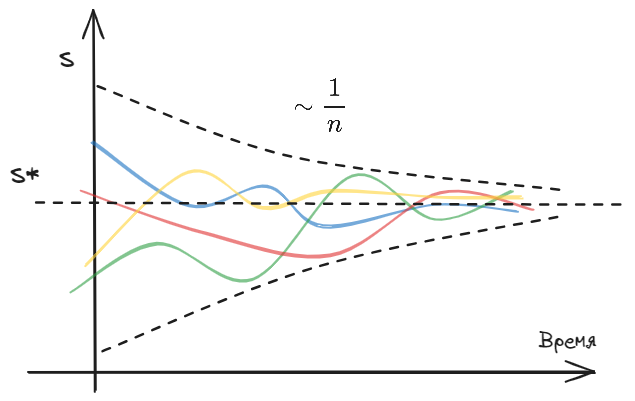
\includegraphics[width=0.9\linewidth]{assets/r-b.excalidraw.png}
    \end{figure}
\end{frame}

\begin{frame}
    \frametitle{RuEdu. Бимодальный корпус образовательных данных}

    \centering

    \begin{block}{Сводная информация}
        \begin{itemize}
            \item Год выполнения: 2024 год
            \item Академический уровень: ВАК
            \item Тема: Обработка данных
        \end{itemize}
    \end{block}  

    \begin{block}{Абстракт}  
        В открытые корпусах текстов на русском языке почти не содержится образовательная тематика. 
        Коллекция состоит из оригинальных собранных данных, включающих текста популярных естественно-научных журналов. 
        Автор также приводит результаты обучения модели на полученном корпусе с помощью низкорангового адаптера,
        существенно снижающего требования к вычислительным ресурсам.
    \end{block}
\end{frame}


\begin{frame}
    \frametitle{Источники данных}
    \centering
    \begin{figure}
        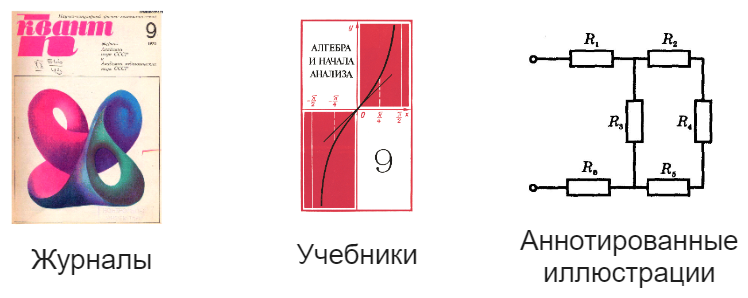
\includegraphics[width=0.9\linewidth]{assets/ruEdu.excalidraw.png}
    \end{figure}
\end{frame}